                 % Chapter Template

\chapter{Situation Assessment} % Main chapter title

\label{chapter:situation_assessment} % Change X to a consecutive number; for referencing this chapter elsewhere, use \ref{ChapterX}

\lhead{Chapter 2. \emph{Situation Assessment}} % Change X to a consecutive number; this is for the header on each page - perhaps a shortened title

In this chapter we introduce the Situation Assessment capacities of our system. Section \ref{sec:situation_assessment-intro} provides an introduction to the subject, with a discussion on some relevant works. Section \ref{sec:situation_assessment-overview} shows an overview of this layer, discussing its key aspects and modules. Sections \ref{sec:situation_assessment-system_inputs} and \ref{sec:situation_assessment-communication} quickly discuss two minor aspects of our implementation, entity detection and communication. In section \ref{sec:situation_assessment-situation_assessment} we explain the geometrical reasoning capacities of our system, showing how symbolic facts are generated, and in section \ref{sec:situation_assessment-belief_management} we show how we build human belief models starting from these facts. In section \ref{sec:situation_assessment-intention_recognition} we introduce our intention recognition module, able to infer the most likely human intentions and actions. Finally, in section \ref{sec:situation_assessment-experiments} we show the experiments conducted to validate this layer, and in particular its intention recognition capacities.

\section{Introduction}
%Motivation
In any application that is not entirely composed by repetitive, precomputed actions, robots need reasoning skills, which severely depend on the quality of the representation of the current environment. This representation can be more or less complex, depending on the application. 

Imagine, for example, a robot whose task is cleaning the floor of a room. In the simplest case, this robot would only be provided with an elementary set of sensors. Without the capacity to understand what areas actually need cleaning, this robot could only move through the room, randomly or with some strategy, achieving the task in a longer amount of time than what would actually be needed. 

% In a fairly simple case, this robot would rely on a map of the room and a set of lasers, or bumper sensors, to detect obstacles. 

Now, imagine a household robot that needs to actively help a family that lives in an apartment, by fetching objects, providing information, and helping to accomplish various tasks. Let us imagine that one of the members of the family, Greg, is moving in the living room, searching around, while exclaming `Where are my glasses?'. In the ideal situation, our robot would try to help Greg, by giving him information such as `They are on the table to your right', or even by fetching them for him. 

Clearly, in this scenario, the robot needs deeper reasoning skills. It needs to understand that the user is looking for its glasses, to link them to their actual physical location, to compute the spatial relationship between the table and the glasses, and to give provide information in a natural way. In fact, if the robot would tell Greg that the glasses are in the position $(3.2, 5.0 , 1.3)$, Greg would very likely be very perplexed. A more natural way would be to inform Greg that his glasses are on a table, whose location is pointed taking into account Greg's position.

In this case, having sophisticated sensors is, of course, important but not sufficient. The robot needs also to \textit{reason} on the sensor's data in order to produce meaningful information. For example: laser points and camera images need to be integrated to recognize objects and humans; spatial relationships  (e.g. the glasses are on the table) have to be properly modeled; actions performed by humans, and their effects on the environment, need to be recognized; and so on. 

The process of reasoning on data to produce symbolic information is called \textit{situation assessment}. Endsley explained in \cite{endsley1995toward} that this process is deeply linked to the quality of  decions of the robot.

While in many applications robots can benefit from a situation assessment component, being able to perform complex reasoning on data is particularly important in HRI. If the robot is able to take better decisions (i.e.  efficient, safe, socially acceptable, natural) than it will be perceived in a more positive manner by humans. 

In the following subsections we will present some important aspects linked to situation assessment.

\subsection{Theory of Mind}
In HRI, it is important to represent humans not as simple obstacles, but as acting entities, with different beliefs on the state of the world and with the capacity to affect the environment. 

A simple example to prove this point is related to proxemics. Normally, when we approach an object, like a table, in an empty environment, we just choose the quickest path. If, intead, the environment is populated by other people, we will follow a set of social rules, like keeping a certain distance from them. If the robot does not follow this rules, it might freighten people, for example by approaching quickly from behind the person, or be considered as `rude'.

Theory of Mind \cite{premack1978does} is a skill used to reason about humans' beliefs and thoughts, and how they affect actions. An ability linked to this concept is perspective taking, which is widely studied in developmental literature.  Flavell in \cite{flavell1977development} describes two levels of perspective taking: 
perceptual perspective taking, the capacity to understand that other people see the world differently \cite{Tversky1999}; and conceptual perspective taking, the capacity to attribute thoughts and feelings to other people \cite{Baron1985}. 

Through perceptual perspective taking we are able to compute information such as `I can see the glasses, but you can not', `you can reach the bottle, but I can not'. Conceptual perspective taking is equally important, and allows us, for example, to understand that a friend, when choosing the flavours for its ice cream, would choose its favourites, which might differs from ours.

An important study linked to conceptual perspective taking is the \textit{divergent belief task}.  Formulated in~\cite{wimmer1983}, this kind of task requires the ability to recognize that others can have beliefs about the world that differ from the observable reality.  In this test, Sally and Ann are two puppets. A short scene is shown to participants, where Sally takes an object and hides it in her box, before leaving the room. While she is away, Anne takes the object from Sally's basket and puts it in her own box. After Sally returns, the participant is asked a question: `Where will Sally look for her object?'. Young children, or those affected by autism, might answer (wrongly) that Sally will look for her object in Anne's box, not taking into account that she does not know that it was moved.

Studies on individuals that do not possess the required mechanisms to perform perspective taking, \cite{frick2014picturing}, have shown that they encounter great difficulties in social relationships,  confirming the importance of this ability.

These studies make us think that perspective taking could be very important in robotics. For example, let us imagine a scenario where Greg and a robot are performing some household repairs, which require the use of different tools. The robot might create a plan to achieve this goal where the human needs to use a screwdriver, which is actually behind a box, hidden from the sight of the Greg. Without perspective taking, the robot will procede in its task while Greg is desperately looking for the screwdriver. By using perspective taking, instead, the robot would infer that Greg does not know where the screwdriver is, and can not see it. In this situation, the robot might inform Greg of the location of the screwdriver, give it to him, or create a plan where Greg does not need to use it, thus being a more likable helper.

Previous works in robotics have actually demonstrated that enhancing the robot's perspective taking abilities improves its reasoning capabilities, leading to more appropriate and efficient task planning and interaction strategies \cite{Trafton2005,ros2010one,breazeal2006}. Let us review some implementations of perspective taking.

The HAMMER, previously presented in chapter ~\ref{chapter-introduction}, system has been extended in \cite{johnson2005perceptual} to introduce perceptual perspective taking, using the concept of forward and inverse visual models. Forward vision models analyze sensory information to produce information, like the geometrical coordinates of objects. Inverse visual models, instead, receive as input desired properties and states (for example, the presence of objects of a certain shape and color in a particular location), and try to produce an appropriate visual image that respects these inputs .

Perspective taking is performed by introducing two forward vision models. The first one produces the location and relationships between objects and end effectors (like grippers), while the second  computes the gaze direction of other agents. Using the results of these models as input of an inverse visual model, the system can reconstruct the scene as seen by another agent. The representation of knowledge by other agents is not explicitly handled in the system. 

~\cite{BreazealGB09}, also presented in ~\ref{chapter-introduction}, is another cognitive architecture which uses simulation mechanisms, but the work  includes both perceptual and conceptual perceptive taking. In this system the robot's schemas are used to build its mental model and execute its tasks, but also to build humans mental models and infer their actions and goal.

The robot is able to build a belief on the world state by analyzing perceptual data, producing symbolic information, such as the location or color of an object. The belief is constantly maintained, by adding new information and erasing those that are no longer valid.
To build a belief model for humans, the robot manipulates perceptual data, by filtering objects that can not be seen by the human (because they are occluded, for example), and transforming the data to simulate a first-person experience on the human. By using the same mechanisms to manage belief for itself and for the humans, the robot can infer divergent belief situations. This method has been tested on variants of the Sally and Anne test with good results.

The belief management algorithm of this systems does not take into account information that can not be directly perceived, but must be inferred. For example, in a domestic scenario, a human might not be aware that a mug containing liquid is hot and should not be touched. These aspects could be inferred by taking into account the results of actions, like pouring hot liquid in the mug.

Another system able to model agent beliefs is ~\cite{scheutz2013computational}. This work is oriented toward problems where a distributed team of agents needs to communicate over a remote connection to solve a task. Each agent is assumed to be able to create its own mental model using its perception capacities, even though the precise rules for these mechanism are not explained. When an agent receives an information, it updates its mental belief using a set of rules, introducing the new data and checking for incongruencies with its previous information.  Using the same mechanism, each agent forms a belief model of other agents that have received the same information.


\subsection{Intention Recognition}
Another crucial skill to interact with humans is recognizing others' actions and goals. This process is is directly linked to modeling humans' beliefs, since, as explained by \cite{byom2013theory} ``as humans, we generally believe that others act in ways that are consistent with their beliefs and goals". In psychology \cite{bruner1981} and philosophy \cite{bratman1984} literature, an intention is the wish and will to achieve a goal. Intentions emerge from contextual causes (motivations) and are present until the goal is achieved or abandoned, pushing agents to undertake actions leading to that goal.

The recognition of human activities is an important topic in computer science research, which can be studied at different levels. Anticipating human actions and movements allows the robot to adapt its behavior and proactively help humans, as studied in \cite{koppula2013anticipating}. 

Sequences of actions can be linked to plans, a well-known topic called plan recognition. Several approaches have been studied in this domain using, for example, classical planning \cite{ramirez2009plan}, probabilistic \cite{bui2003general} or logic techniques \cite{singla2011abductive}.

Other approaches that can be used to estimate the intention of a human are Interactive Partially Observed Markov Decision Processes (I-POMDP) and Inverse Learning. I-POMDP  \cite{gmytrasiewicz2004interactive} offer a rich framework that extends Partially Observed Markov Decision Processes (POMDP) in a multi-agent setting. Inference in these models can be extremely complex, but there have been attempts at solving this issue, like in \cite{doshi2009monte,hoang2013interactive}. 

Inverse Reinforcement Learning \cite{ng2000algorithms} formulates the problem of computing an unknown reward function of an agent after observing his behavior. This strategy has been applied, with Bayesian Networks (BN), in \cite{Nagai2015}, in order to learn the mental model of another agent, and choose appropriate actions for a relationship building task. A linked approach is inverted planning, which has been applied in a bayesian framework in \cite{baker2009action}  for human action understanding.

The use of contextual information can be used to further disambiguate complex situations. \cite{Liu2014} shows a system using BNs to understand users' intentions with an emphasis on contextual information. This BN is constructed using object affordances nodes (e.g. a cup can be used for drinking or washed), context nodes (e.g. it's a hot day, the cup was recently used), and intention nodes (e.g. drinking from a cup or washing it). The causal links between contexts and intentions are learnt through a user study, which uses an online questionnaire where participants need to rate the strenght of the connection betwen an intention and a context. The work does not study how to adapt this this BN to complex plans, composed by sequences of actions.

It is very important to consider humans' beliefs when estimating their intentions. In a dynamic environment, agents can execute actions, modifying the state of the world without other agents being able to perceive the changes. Let us imagine a scenario. Bob comes back home from work and would like to relax while reading. He lays down on a sofa with a book, and reaches to a nearby table to grab his glasses. He does not know that his wife, during the day, moved the glasses to another room. If we would ignore Bob's beliefs on the world (i.e. he does not know that the glasses are not on the table) we could infer that, for example, Bob would like a drink while he is sitting on the sofa, or the tv remote controller. If, instead, we would know that Bob thinks his glasses are on the table (and we would use other contextual information perhaps, like Bob's habitudes) we would be able to correctly infer Bob's current intention, that is, taking his glasses, and warn him that they are not there, perhaps even fetching them for him. 

In robotics, an interesting framework that considers this issue is the Bayesian Theory of Mind \cite{baker2014modeling}, used to represent the inference process of an observer looking at another agent's behaviors. The acting agent is modeled as a POMDP, whose richness is able to represent its possible beliefs about the world. The observer's process is modeled as a DBN, built starting from the agent's POMDP but considering his reward function (that represents his desires) as hidden. The system has been tested against some alternative models and compared, in user studies, with human capacities, to understand how well it models theory of mind. Since the models used are quite complex, scalability in the model could be an issue. Also, the study is focused on a single-agent scenario, and does not consider collaborative problems.

Let us examine the two simulation-based systems that we already presented in the previous section, HAMMER ~\cite{demiris2007prediction}, and the architecture of \cite{BreazealGB09}, and see how these cognitive architectures are able to infer actions and intentions.

The HAMMER system is organized with couples of inverse and forward models.  Inverse models receive as input the goal and state of the system, producing the motor commands which are needed to achieve the goal. Forward models, instead, receive as input motor commands and compute the predicted future state. When these two models are linked, the forward model receives as input the motor commands produced by an inverse model. This link can form a loop, with the output of a forward model returning to its inverse model, which can adjust a range of parameters if the predicted future state does not match exactly the desired state. These models can be organized in parallel schemas and used to recognize actions performed by a demonstrator. 

In this case, the demonstrator's current state, as perceived by the robot, is fed in the inverse models, which in turns sends their output to their forward models. The state predicted by the forward models are compared with the demonstrator's state at the next time step. This comparison produces a score, which can be used to infer the most likely action performed. 

Forward and inverse models can be organized in hierarchical schemas, to infer actions and plans. The complexity of these schemas could be quite significant, particularly when trying to recognize a goal which can be achieved in many different ways, depending on the context. 

\cite{BreazealGB09} uses a similar ideas, where the all the possible robot movements are represented as a graph of connected poses, with arcs representing possible transitions between the poses. This schema is used both to represent the robot's movements and to map observed trajectories. Tasks are represented as schemas, which can be organized in sequential and hierarchical structures to represent complex goals.

 When trying to infer an agent's intention the robot tries to find a schema whose motor action matches the observed activities of the agent. After that, the schema is traversed in reverse in order to try to determine the real intention. The system is not able to deal with ambiguities, and this algorithm stops if it comes to a point where there is more than a possible explanation for the current behavior. 

An example of non simulation-based system in this topic can be seen in \cite{talamadupula2014coordination}. This architecture is used to coordinate human-robot teams, based on intention recognition and belief modeling. Creating and maintaining beliefs is handled using the strategy explained in ~\cite{scheutz2013computational}, presented in the previous subsection. Prediction of other humans intentions is based on the plan recognition algorithm of \cite{ramirez2009plan}. While this algorithm uses efficient replanning to increase its efficiency, in complex domains, where the users have many different strategies to achieve a goal, the system would need to execute frequent replans to infer the actual strategy chosen by the user, which can be expensive.

\section{System Overview}
\label{sec:situation_assessment-overview}

In our architecture, we built a Situation Assessment layer, which is able to:
\begin{itemize}
\item  Detect and track humans and object.
\item  Process sensor data in order to produce symbolic information, such as spatial relationships between objects and humans.
\item  Maintain a belief model for each agent, which includes their current knowledge on the environment.
\item  Infer human actions and intentions. Our system is able to perform this estimation by taking into account the current belief models of the humans. 
\end{itemize} 

Before detailing this layer, we will introduce a number of definitions:
\begin{itemize}
\item Agent. We consider as agents both humans and robots.
\item Entities. We call entity an agent or an object.
\item Fact. A fact is a tuple $(subject\> predicate\> value)$, which we use to represent symbolic knowledge. An example of fact is $(CUP\> isOn\> TABLE)$ to define the location of an object. 
\item World State. A collection of facts that describes all the information about current situation that are considered relevant for the system. The world state will include, for example, the symbolic position of objects and agents.
\item Belief Model. A collection of facts representing the knowledge of an agent on the world state. Each agent can have a different belief model, since the environment can change without an agent being able to perceive it. For example, the robot could take a tool from the table, while Greg is in another room, and place it in a box. Greg has not seen this event, and so his belief model will contain the (wrong) information that the tool is still on the table.
\end{itemize}

We can assign \textit{attributes} to entities, parts of entities (e.g. the arm of a human), and areas to represent different information, like properties, the state of entities or relationships between entities. Examples of attributes are:
an agent can be in a specific area; a box can be opened and can contain objects; a bottle can contain liquids; a mug can be hot; a room can be a silent area, where the robot should avoid making any noise.
We divide attributes in two classes, which influence the capacity of agents to perceive them: 
\begin{itemize}
\item Fully observable. These attributes can be observed by any present agent looking at the linked entity or area (e.g. the box is open, Greg is in the kitchen).
\item Partially observable. These attributes can be observed by present agents only in specific situations, represented as rules linked to the object and the attributes, e.g. an agent can see that a box contains items only when it is open, an agent can detect that the mug is hot only when he touches it. 
\end{itemize}

The instance of an attribute is represented as a fact, and so, each fact will corespond to exactly one attribute. Section ~\ref{sec:situation_assessment-belief_management} will show how we actually compute if an agent is able to perceive an attribute, and how we update his belief model. 


\begin{itemize}
\item Sensor Data. Data produced by different possible sensors (e.g. lasers, camera, etc.).
\item Entity Detection. Different components detect and track humans and objects in the environment.
\item Human Inputs. Users can communicate with the robot by using a tablet application.
\item Human Interface. User inputs from the tablet are elaborated into commands, to be introduced in the be Database.
\item Geometrical Reasoning. Symbolic facts are produced starting from perceptual data.
\item Belief Management. The system maintains a mental model of each agent.
\item Intention and Action Recognition. Human actions and intentions are inferred based on information provided by the Geometrical Reasoning and on the belief models of the agents.
\item Database. The Database stores symbolic facts produced by the system.
\end{itemize}


 \begin{figure}[ht!]
	\centering
	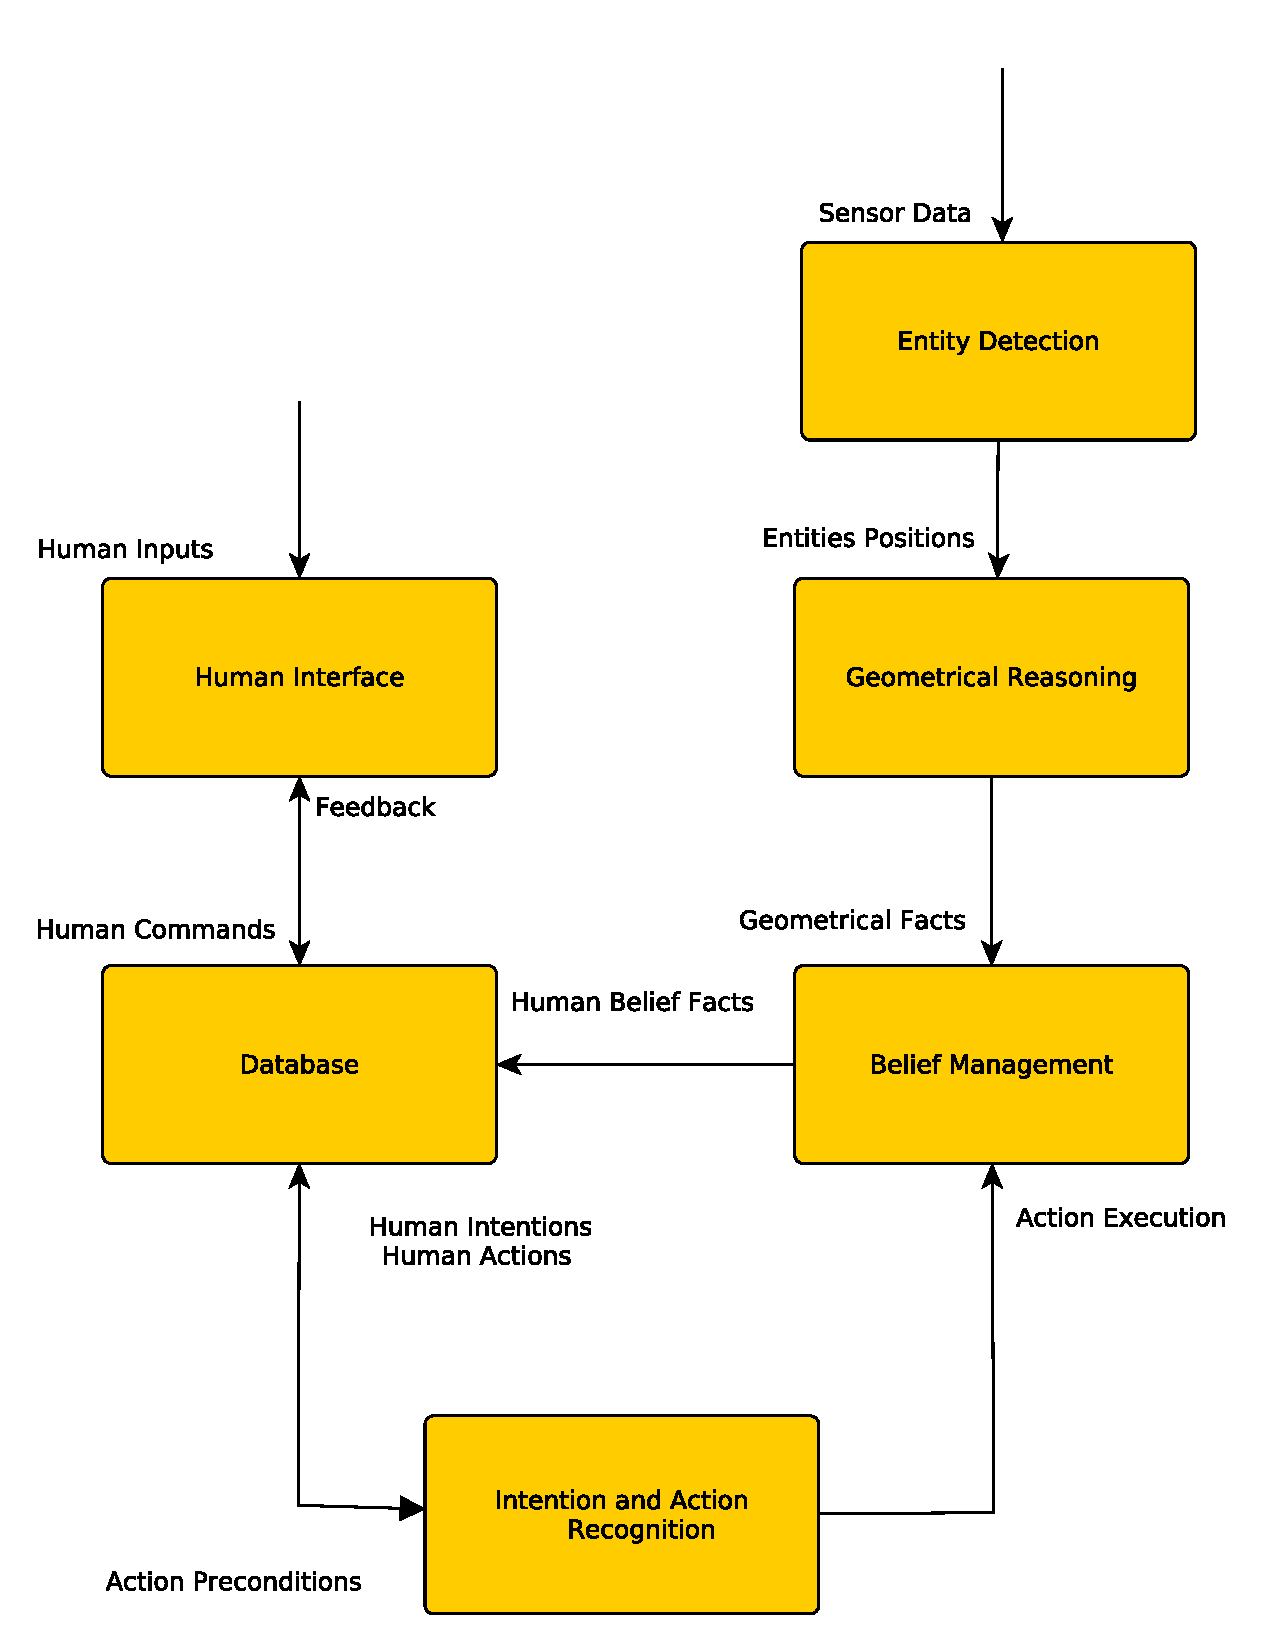
\includegraphics[scale=0.45]{img/situation_assessment/situation_assessment_overview}
	\caption{Overview of the different modules composing the Situation Assessment layer}
	\label{fig:situation_assessment-situation_assessment_overview}
\end{figure}

In addition, we introduce a description of the world, with a definition of all the elements known to the robot, like objects and agents, possible actions, possible intentions, etc. 

Symbolic facts are constantly produced, starting from the sensor data and from the position of entities. The Belief Manager collects these information to maintain the belief model of each agent. The belief model of humans and of the robot is used by the Intention and Action Recognition module to infer the most likely human intentions, and which actions they perform. All these information are introduced in the Database, and can be read by other components. For example, the Goal Management layer can choose a goal based on human commands or an estimation of humans' intentions. In a similar way, the Execution Management layer will read the Database in order to obtain the state of the world, to check action preconditions.  

The geometrical reasoning and belief management capacities of this layer were presented in \cite{Milliez2014}, where they were used to pass the Sally and Anne test~\cite{Baron1985} on a robotic platform. The intention and action recognition skills of the system were introduced in \cite{devin2016some}.

Dialogue can be a very important source of information. Agents often communicate, while executing a task together, or even when working independently, to clarify ambiguities and obtain missing information. While we will not present a specific dialogue component in this work,  in \cite{Ferreira2015} our belief management component was integrated with a situated dialogue system in a simulator. This model was compared with a basic system (without belief awareness) in a study with 60 interactions, in a simulated environment. We successfully showed that the dialogue management system significantly improves its efficiency, reducing the number of dialogue turns in the interaction, and its accuracy, with a higher success rate when a divergent belief situation appears.

In the following sections we will introduce the most important aspects of the Situation Assessment Layer.

\section{System Inputs}
\label{sec:situation_assessment-system_inputs}
In our system, we chose to simplify perception issues, focusing on reasoning aspects. We associate a unique tag to every object that is interesting in a particular scenario.  When the robot observes a tag using a camera, it detects the corresponding object using a tag-matching algorithm.
Regarding humans, we use a motion capture software to identify and track agents moving in the environment. Using different tags, we can track the head, shoulders, and right arm of a human. Our situation assessment component has also been tested using a laser and RGB based detector in the SPENCER european project~\cite{lindermulti}.

 \begin{figure}[ht!]
	\centering
	\includegraphics[scale=0.7, trim={0 3cm 0 0}]{img/situation_assessment/explore.pdf}
	\caption[The robot builds a representation of the environment]{The robot explores the environment, recognizing objects through tags, and building a representation of the environment.}
	\label{fig:situation_assessment-explore}
\end{figure}


Similarly, communication between the human and the robot is limited, in our system. Humans can give commands to the robot by using a tablet application, where they can manage the robot goals, by adding a new goal, canceling a previous one, or pausing the robot. Requests are added to the Database, and can be read by the Goal Management layer. 

 \begin{figure}[ht!]
	\centering
	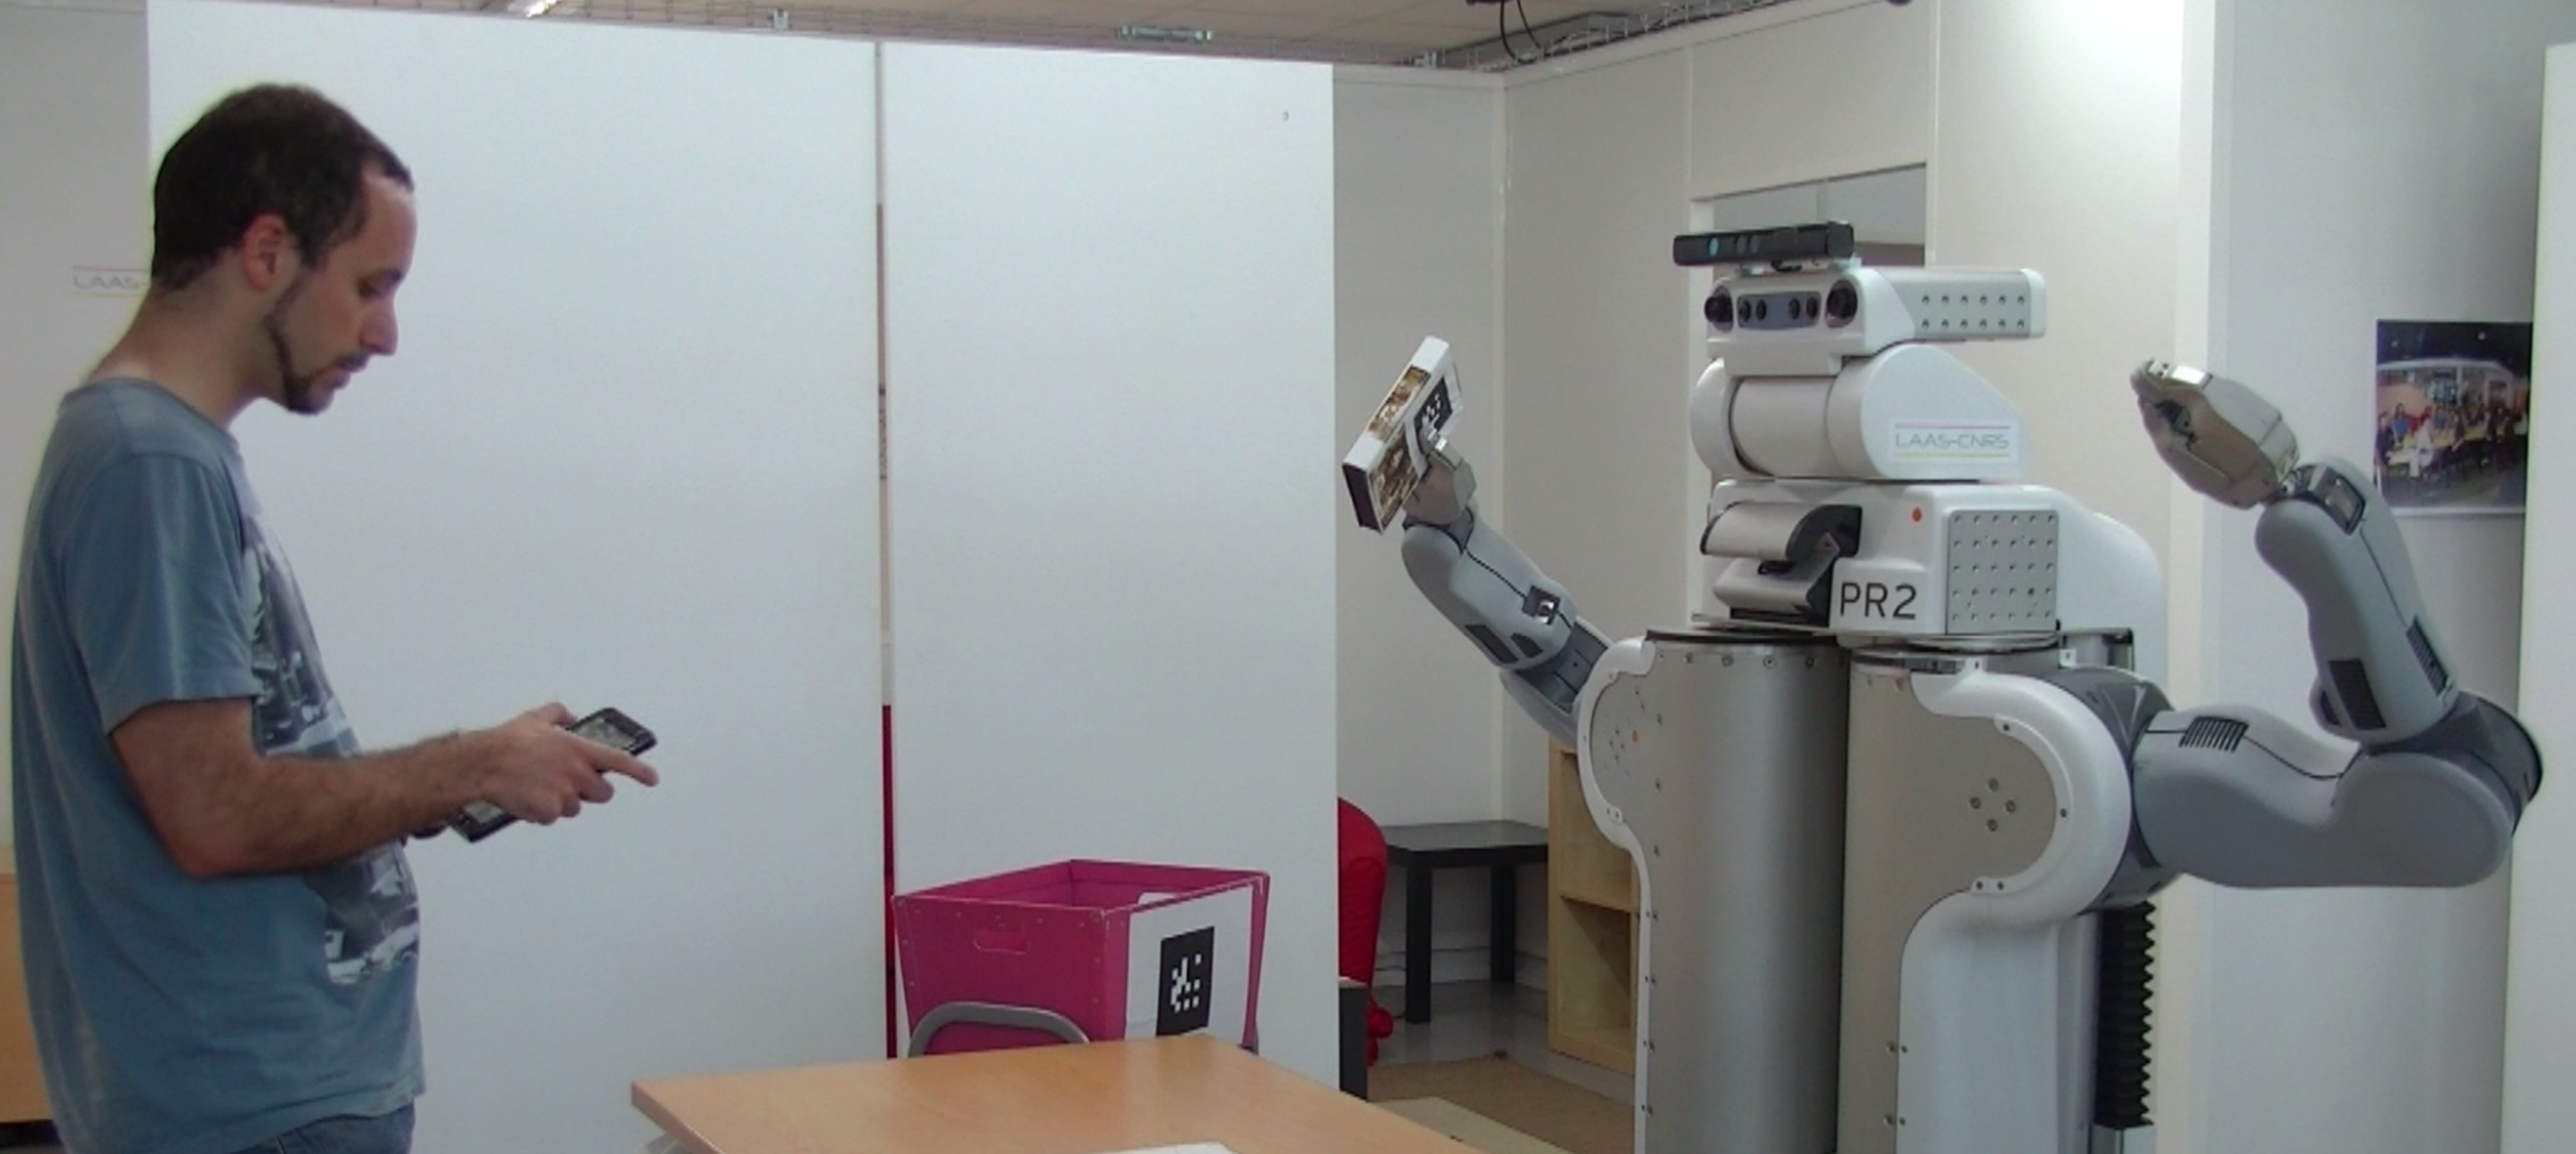
\includegraphics[scale=0.2]{img/situation_assessment/tablet.pdf}
	\caption{Using a tablet to interact with the robot}
	\label{fig:situation_assessment-explore}
\end{figure}

\section{Geometrical Reasoning}
Using its perception abilities the robot can build a representation of the environment, starting with entities' positions. Using geometrical reasoning we can compute spatial relationships between entities, e.g. the glasses are on the shelf, the human is moving toward the library, the glasses are reachable by the human, the bottle is visible for the human. These reasonings provide a base for the perspective taking abilities of the robot.  The Geometrical Reasoning capacities of our system were introduced in ~\cite{Sisbot2011}. This work was updated to include the production of new symbolic facts. We will show a list of some of the most important facts that our system is able to produce through geometrical reasoning.

\begin{itemize}
\item isOn. Used when an object is on top of another, for example $(CUP isOn TABLE)$.
\item isNextTo. Used when two objects are on the same surface and close to each other, for example $(CUP isNextTo BOX)$.
\item isReachable. Used when an object is reachable by an agent, computed through inverse kinematics. An example of such predicate is $(CUP isReachableBy ROBOT)$
\item isVisible. Used when an entity is visible by an agent. This is calculated by computing the field of view of an agent, and checking if there is a sufficient portion of the object not hidden by occlusions in this field. An example of this predicate is $(CUP isVisibleBy ROBOT)$.
\item isMoving. Used when an agent is currently moving. This is computed by checking if the agent's displacements in a pre-determined time unit is bigger than a pre-determined threshold. We use an hysteresis filter to avoid continuous changes in the value of this fact. An example of this fact is $ROBOT isMoving TRUE)$.
\item isMovingToward. This fact indicates that an agent is moving toward a particular entity. This is computed by checking if the distance between the agent and the entity is decreasing. An example of this predicate is $(ROBOT isMovingToward GREG)$.
\item isOrientedToward. This fact indicates that an agent is oriented toward a particular entity, for example $(ROBOT isOrientedToward GREG$).
\item pose. This fact indicates that an agent is in a particular pose, for example $(GREG pose HANDOVER)$.
\end{itemize}


\section{Belief Management}
\label{sec:situation_assessment-belief_management}
In our system, agents can have divergent representations of the world. To model this aspect, the information produced by perception, geometrical reasoning and inference, are collected by the robot in \textit{belief models}, built for itself and for each agent. A belief model is a symbolic representation of the world state, as known by an agent. In a model, the world state is represented by a list of facts. To represent the lack of knowledge of an agent, the value of a property can be \textit{unknown}.

We consider our world as a dynamic environment, where attributes can change and actions can be performed.  We define an \textit{action} as a tuple $(name, preconditions, target, postconditions)$. The $name$ of an action is a unique string that identifies it. The $preconditions$ are a set of facts that must be true in order to realize the action. In our system, an action is executed on a $target$, which can be a physical object, like a cup, but also an area of the environment, like a room. The $postconditions$ are the set of facts, and their values, affected by the action's execution.

Since we are interested on reasoning and not perceptual aspects, we use inference, as explained in Sec. \ref{sec:situation_assessment-intention_recognition}, in order to understand when a human has performed an action. Through the predefined $postconditions$ of actions we can also infer changes in the state of objects, e.g. the human opens a box, so the box is now open. 

We have created a rule based framework in order to build the beliefs of each agent and update them when needed. Human belief models are updated using the perspective taking skills of the robot. When the robot detects the execution of an action in the world, with the mechanisms shown in section ~\ref{sec:situation_assessment-intention_recognition}
it updates the belief model for itself and for every human that can perceive the action, adding the action's $postconditions$ to their models. When an action is not perceived by a human (e.g. the user was in an other room), his belief model will not be updated, as he is not aware of the changes that occurred.

However, when he comes back and looks at the environment, we assign him a new belief state following a set of rules, which we will now explain. We call $H$ the agent, $HB$ his belief model, and $RB$ the robot's belief model. We also create the following predicates: $obs(p)$ means that $p$ is observable for $H$, $valid(p,x)$ means that $p$ does not contradict the current perception data of agent $x$, $value(p,m)$ is the value $p$ in belief model $m$, and $vis(p,x)$ means that agent $x$ has visibility on the linked entities of $p$. The rules for the $valid$ predicate will be different in each attribute. For example the fact \textit{MUG isOn TABLE} will not be valid for agent Max if he can see that there is no mug on the table. For each fact $p\in HB \cup RB$:
\begin{itemize}
\item if $p \in RB, \quad p\not\in HB,\quad obs(p),\quad vis(p,H) \rightarrow value(p,HB)=value(p,RB)$.
\item if $p \not \in RB,\quad p\in HB,\quad obs(p),\quad vis(p,H) \rightarrow remove\quad $p$ \quad from \quad HB$.
\item if $p\in RB,\quad p\in HB$ then:
	\begin{itemize}
      \item if $value(p,HB)\neq value(p,RB),\\ \quad obs(p),\quad vis(p,H) \rightarrow \\ value(p,HB)=value(p,RB)$.
      \item if $value(p,HB)\neq value(p,RB),\\ \quad !obs(p),\quad !valid(p,H) \rightarrow \\ value(p,HB)=\textit{unknown}$.
	\end{itemize}
\end{itemize}
The idea of this set of rules is updating an agent's mental belief model for a property only if it's observable, or if it's not observable and perception data contradicts the current value of the property (e.g. the mug was moved from the table to the kitchen while the agent was in another room: while the agent can not see where is the mug, he can see it is no longer on the table).


%TODO: Image of perspective taking

\section{Intention and Action Inference}
\label{sec:situation_assessment-intention_recognition}
Understanding what others are doing is an important skill for a robot partner. We have designed a module that is able, through inference, to recognize human actions and connect them to possible intentions. Actions and intentions are evaluated with perspective taking using the humans' belief models, and further disambiguated by taking into account the current context.

In order to perform this reasoning, we will provide the following information to the robot: a list of known contexts, a list of known intentions, a list of known actions, a set of observations of human actions, and a belief model of humans and of the robot itself.

We propose, as central model used for intention estimation, a framework based on BNs. We call our implementation of BN an Intention Graph (IG).
An IG is linked to a specific agent, and composed by the following layers of nodes:
\begin{itemize}
\item Context Nodes: these nodes represent contextual information, modeled as boolean variables (e.g. HotDay, ColdDay).
\item Intention Nodes: these boolean nodes represent the set of possible intentions. Each intention can conditionally depend on several contexts.
\item Action Nodes. This is the set of human actions whose preconditions are satisfied when the IG is created. Each of these nodes is conditionally dependent on all the intention nodes. 
\item Observation Nodes. We associate to each action a different set of observation nodes, that depend conditionally on the associated action node. 
\end{itemize}

In a typical usage, the robot will create, for each monitored human, an IG, formed by the Context and Intention Nodes, which we consider statically known by the robot, and a variable list of Action and Observation nodes, which depends on the human's belief model. The robot will create action nodes for each known action whose $preconditions$ are satisfied in the human's belief model, and their related Observation Nodes. These IGs will be updated every time that an agent performs an action, creating and removing Action and Observation nodes, depending on the state of the world after the action was performed.

When monitoring a human, we set Context Nodes and Observation Nodes as \textit{evidence}, considering them observable by the robot. These information will allow us to have a good estimation of the most likely actions and intentions of the human, as explained in subsection \ref{sec:situation_assessment-intention and action inference}. 


An example of IG, taken from an experiment, can be seen in figure \ref{fig:situation_assessment-intention_graph}. In the following paragraphs, we will explain the role of these layers of nodes, and how the conditional dependencies between them are computed.

 \begin{figure}[ht!]
	\centering
	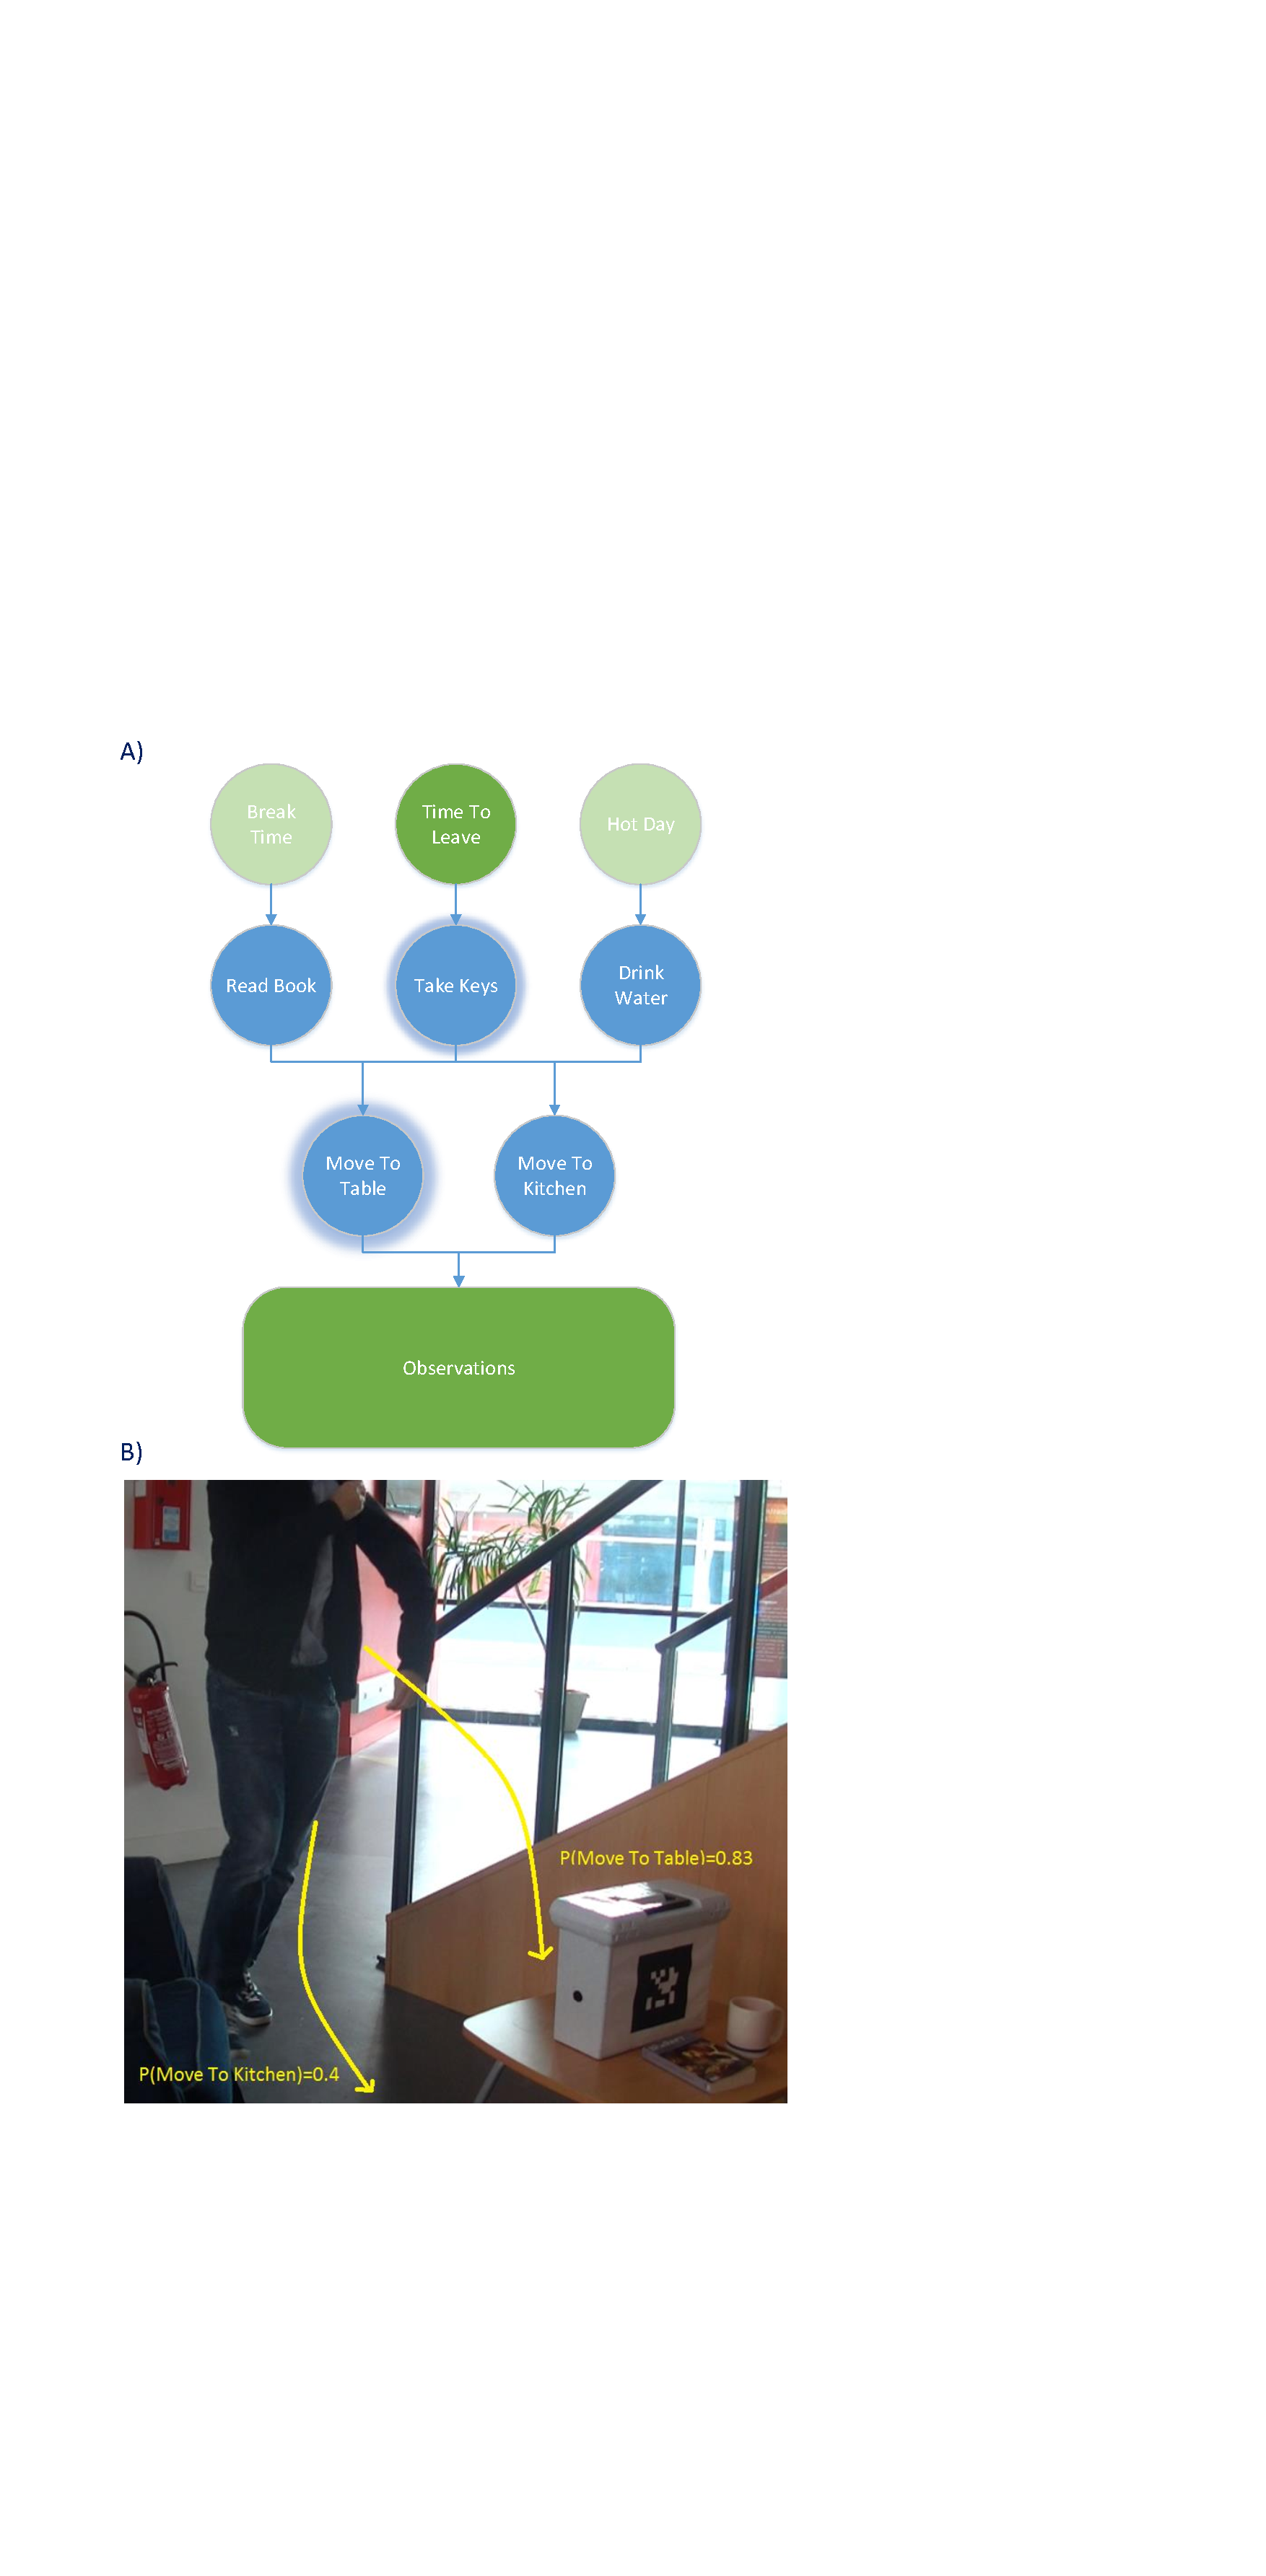
\includegraphics[trim={2cm 11cm 11cm 17cm},clip,scale=0.45]{img/situation_assessment/cookieScenario.pdf}
	\caption[Intention Graph]{A scene from our experiment. The yellow arrows show possible actions and their associated probabilities. The diagram represents the current IG. Green circles represent evidence nodes and blue circles other nodes. For the Context Nodes (top of the graph), we represented nodes with a false value as greyed out, and nodes with a true value as green. The most likely nodes in the graph are represented with a glowing effect. The observation nodes were compressed in a single block to simplify the diagram}
	\label{fig:situation_assessment-intention_graph}
\end{figure}

\subsection{From Contexts to Intentions}
We introduce a set of contexts in our domain. We consider as context any information that can be used to characterize and motivate an intention \cite{abowd1999towards}. We model a context  as a fact, which can assume different values and influences the probability of a user having a particular intention. For example, we imagine that a human is more likely to be cooking at dinner time, or to drink a hot mug of tea on a cold day.

Contextual nodes can directly influence one or more Intention nodes. In this work, we chose to learn these conditional dependencies from humans, as explained in section \ref{sec:situation_assessment-experiments}.

\subsection{From Intentions to Actions}
\label{sec:situation_assessment-action_evaluation}
To understand how actions are linked to intentions the robot needs to answer the following question: what actions would a human take, in this situation, given his belief of the world, in order to achieve its intention?
Our idea is based on the principle of rationality \cite{Dennet1989}, which states that agents tend to choose the most efficient actions, taking into account their beliefs about the world, in order to achieve their desires.

In \cite{Blakemore2001}, the authors explain that ``the attribution of intentions to actions might rely on simulating the observed action and mapping it into representations of our own intention". We represent this idea by providing the robot with a set of planning models. Each one of these planning models is related to an intention, and represents all the known plans to achieve its linked goal. In this way, we can estimate how much the current human actions are compatible with the plans related to an intention.

In our implementation, for each intention known by the robot, we will create an associated Markov Decision Process (MDP), to represent all the possible plans linked to this intention. After solving the set of MDPs we will use the calculated action value function \(Q(s,a)\), to create conditional dependencies between Intention and Action nodes in the IG. Let's start by defining \(P(a|I_i=1)\), the probability that action $a$ will be performed if intention $I_i$ is true. We model this probability as:
\begin{equation}
 P(a|I_i=1)=\frac{Q_i(s,a)}{\sum_b(Q_i(s,b))}
\end{equation}
  where we normalize the value function $Q_i(s,a)$ for intention $i$ and action $a$ in the human's belief state $s$, over the value function $Q_i(s,b)$ calculated on all the monitored actions $b$. We can extend this calculation to the case where a generic number of intentions are true to compute the probabilities of action nodes: 
\begin{equation}
  P(a|I_1,I_2,...,I_m)=\frac{\sum_{i:I_i=1}Q_i(s,a)}{\sum_b\sum_{i:I_i=1}Q_i(s,b)}
\end{equation}

The key idea in this problem is to use the human's belief state as input for the MDPs' value functions. In this way we are using perspective taking at a planning level, since the human action will be consistent with his intention in his own belief state but may be not optimal, irrelevant, or even dangerous in the real world (e.g. in case of wrong belief).

Our idea is similar to \cite{karami2010human}, where human intentions are estimated using a POMDP and a set of MDPs, that simulate human policies related to different intentions. In this work we use a BN instead of a POMDP, which allows us to separate the mechanisms used for inference and for the robot's actions. Also, we improve the recognition process by including the belief state of the human.

\subsection{From Actions to Observations}
Intentions will be inferred from human actions, so the robot needs to monitor their execution. For each Action Node we define a set of four Observations Nodes: the distance of the human's body from the action's $target$, its variation, the distance of the human's hand from the action's $target$, and its variation. The conditional dependencies of the Observation Nodes are precomputed.

\subsection{Intention and Action Inference}
\label{sec:situation_assessment-intention and action inference}
We assume, in this work, that at each moment a human can only execute a single action, and the robot will react only to his most likely intention. The most likely action and intention are inferred from the BN in the following way. We call $P(n)$ the inferred probability of a node $n$, $B(n)$ the set of brothers of $n$ (that is, nodes on the same layer), and $\delta_1$, $\delta_2$ two thresholds. The robot infers that an action has been realized, or that a human has an intention, following these rules: 
\begin{itemize}
\item  \(P(n_i)>\delta_1\) 
\item  \(\forall b \in B(n_i): P(n_i)>P(b)+\delta_2\), where $n_i$ is the node associated to the interested intention or action.
\end{itemize}

When the robot infers that an action has been performed, it updates the world state with its $postconditions$, triggering an update on the beliefs of all present agents. The current human intention is recorded in the Database, and will be used by the Goal Management layer.

 \begin{figure}[ht!]
	\centering
	\includegraphics[scale=0.8, trim={0 4cm 0 0}]{img/situation_assessment/pick.pdf}
	\caption[Actions and world update]{The human picks an object and the robot updates accordingly the world state. The spheres surrounding objects show when the human's hand is considered to be near an object.}
	\label{fig:situation_assessment-pick}
\end{figure}


\subsection{Proactive Behaviors}
\label{subsec:situation_assessment-proactive_behaviors}
Information about the most likely intention and action will be introduced in the database, to be read by the Goal Management Layer. Based on this information, the robot can execute two different proactive behaviors: correcting the belief state of the human, and proactively helping him to achieve his task.

\subsubsection{Correcting Belief State}
Having a wrong or incomplete belief on the world state can lead agents to execute non optimal, useless, or even dangerous actions. The robot needs to detect these situations in order to warn the human. The robot assumes that it always holds a correct belief state. Our solution uses the expected action rewards introduced in \ref{sec:situation_assessment-action_evaluation}. The idea is comparing the expected reward for performing an action according to the human and the robot's belief states. To formalize: we compare the action values \(Q_m(s_h,a_h)\) and \(Q_m(s_r,a_h)\), where $m$ is the most likely intention,  $s_h$ and $s_r$ are the robot's and human's belief state, and $a_h$ is the most likely action. If these values are not equal the human expects a different outcome from its action than what should actually happen. 

We propose a simple solution, where the robot warns the human of the detected divergent belief for that action. For example, Bob wants to drink tea from a closed, opaque bottle, which the robot knows is empty (perhaps because another agent drank the last glass), while Bob does not. When he approaches the bottle, the robot detects that his most likely intention (using the process described in section \ref{sec:situation_assessment-intention_recognition}) is to drink tea. The system calculates the expected rewards from taking the bottle in the two belief models and obtains different values. The system checks the facts related to the attributes associated to the bottle in the two mental models, and extracts the differences. Using this information, the robot corrects the divergent belief, informing the human that the bottle is now empty. 

In our system, the Goal Management layer will detect these situations, by reading the Database, and choose a \textit{warn agent} goal (as will be explained in chapter \ref{chapter:goal_management}).

\subsubsection{Performing a part of the plan}
There are situations in which the robot should help the human achieve its goal by physically acting. The Goal Management layer will consider new inferred intentions as possible goals for the robot, and will communicate with the Plan Production and Management layer to achieve them, as explained in chapters \ref{chapter:goal_management}, \ref{chapter:plan_management}, and \ref{chapter:plan_execution}. 


\section{Experiments and Discussion}
\label{sec:situation_assessment-experiments}
\subsection{Case Study}
Evaluating the capacity of the system to estimate human intentions is not easy, since intentions are not directly observable. A possible solution, as shown in \cite{baker2014modeling}, is comparing the estimation of human intentions, performed by other humans, with the predictions of our system. In order to perform this comparison we created a user study where we showed participants several videos, asking them to estimate the likelihood of a set of intentions for each video, and collected their results. 

We performed an equivalence test, comparing users' intentions predictions with those of the robot, following the two one-sided tests (TOST) approach. We choose as a threshold for equivalence the standard deviation $\sigma$ of the users' answers. The idea behind this choice is that, if the robot's answers are closer than a standard deviation to the average human answers, its predictions are comparable to an average human answer from our user group. 

We defined our hypothesis as follow: 
\begin{itemize}
\item $H_0$: $\mu_{hi}-\mu_{ri}\leq-\sigma_{hi}$ OR $\mu_{hi}-\mu_{ri}\geq\sigma_{hi}$ 
\item $H_A$: $-\sigma_{hi}<\mu_{hi}-\mu_{ri}<\sigma_{hi}$  
\end{itemize}
where $\mu_{hi}$ and $\mu_{ri}$ are the human average and the robot's answer for test $i$, $\sigma_{hi}$ is the variance of the human answers for test $i$.

We performed tests to evaluate: a) prediction in absence of clues, b) prediction in the presence of contextual clues, c) prediction in the presence of belief state clues.

We built a household environment with a fixed set of furniture: a \textit{Kitchen Shelf}, a \textit{Table}, a \textit{Sofa}, and a \textit{Chair}. In this environment, we created two scenarios, composed by several tests, with two agents, \textit{Max} and \textit{Bob}, performing different actions. Each scenario contained a set of objects, and a constrained set of intentions. For the tests related to belief states, we start by showing the users and the robot a specific sequence of events, allowing them to build a mental model of the agents. We will describe in details the two scenarios and the relative tests.

\subsubsection{Cookie Scenario}
\begin{itemize}
\item Objects: a \textit{Cookie Box}, a \textit{Mug}, and a \textit{Bottle of Water} were placed on the \textit{Table}, close to each other. A pack of \textit{Cookies} was placed on the \textit{Kitchen Shelf}. The \textit{Cookie Box} could contain, or not, \textit{Cookies}.
\item Intentions: \textit{Eating a Cookie}, \textit{Drinking Water}, \textit{Reading the Book}.
\item Tests:
\begin{itemize}
	\item \textit{No Clues}: \textit{Max} approaches the \textit{Table}.
    \item \textit{Contextual Clues}: \textit{Max} approaches the \textit{Table} commenting on the warmth of the day.
	\item \textit{Divergent Belief Max}: \textit{Max} approaches the \textit{Table}.
	\item \textit{Divergent Belief Bob}: \textit{Bob} approaches the \textit{Table}.
\end{itemize}
\item  \textit{Divergent Belief Event}:  \textit{Max} and \textit{Bob} are chatting on the \textit{Sofa}. Max eats the last \textit{Cookie} from the \textit{Cookie Box} before closing it and leaving. While \textit{Max} is away, \textit{Bob} takes \textit{Cookies} from the \textit{Kitchen Shelf}, fills the \textit{Cookie Box} with them, and closes it, before leaving.
\end{itemize}

The \textit{Divergent Belief Event} was shown to the users and the robot between the \textit{Contextual Clues} and the \textit{Divergent Belief Max} events. 

We deliberately included an intention, \textit{Reading the Book}, without placing a book in the visible environment, introducing a confusing element in the scenario. This scenario can be seen in figure~\ref{fig:situation_assessment-cookie}.


 \begin{figure}[ht!]
	\centering
	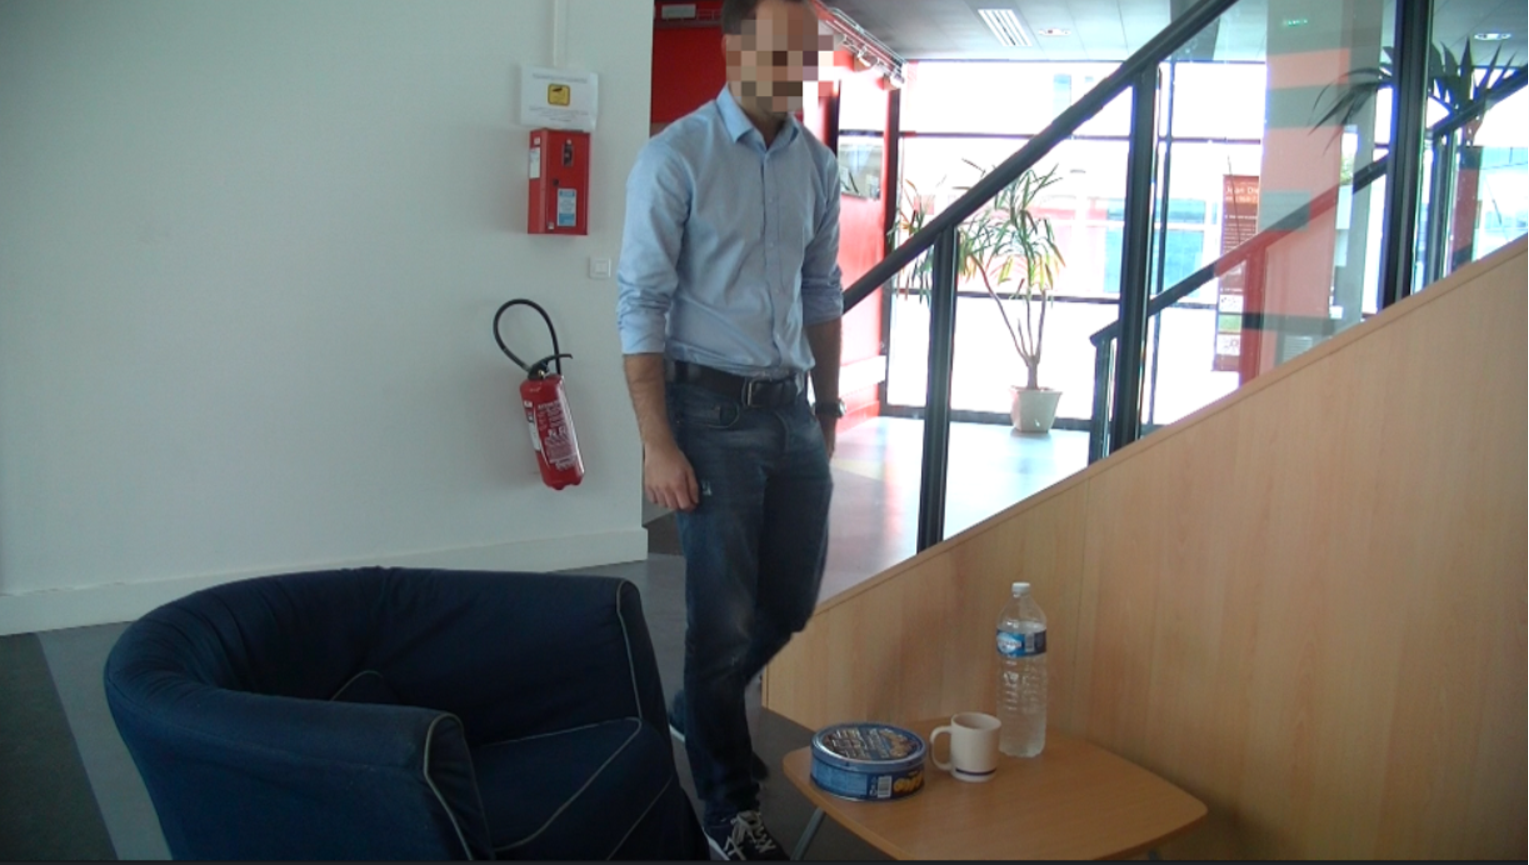
\includegraphics[scale=0.5]{img/situation_assessment/cookie1-blur.pdf}
	\caption{The cookie intention scenario}
	\label{fig:situation_assessment-cookie}
\end{figure}


\subsubsection{Keys Scenario}
\begin{itemize}
\item Objects: A \textit{Box} was placed on the \textit{Table}, that partially occluded the sight of people approaching. A \textit{Book} and a \textit{Mug} where placed behind the \textit{Box}, so that they could be seen from the sofa but not from approaching people.
\item Intentions: \textit{Taking the Mug}, \textit{Taking the Keys}, \textit{Reading the Book}.
\item Tests and Events:
\begin{itemize}
\item \textit{No Clues}: \textit{Max} approaches the \textit{Table}.
\item\textit{Contextual Clues}: \textit{Max} approaches the \textit{Table} in a hurry, while putting on a coat.
\item \textit{Divergent Belief Max}: \textit{Max} approaches the \textit{Table} in a hurry, while putting on a coat.
\end{itemize}
\item \textit{Divergent Belief Event}: \textit{Max} is sitting on the \textit{Table}, drinking from the \textit{Mug}, while having the \textit{Keys} in his hands. His phone rings, so he drops the \textit{Keys} and the \textit{Mug} on the \textit{Table}, behind the \textit{Box}, and leaves the room. While \textit{Max} is away, \textit{Bob} comes and sits on the \textit{Sofa}, reading a \textit{Book}. When he sees the \textit{Keys}, he takes them, places the \textit{Book} on the \textit{Table}, and leaves.
\end{itemize}

The \textit{Divergent Belief Event} was shown to the users and the robot between \textit{Contextual Clues} and the \textit{Divegent Belief Max} events. This scenario can be seen in figure~\ref{fig:situation_assessment-keys}

 \begin{figure}[ht!]
	\centering
	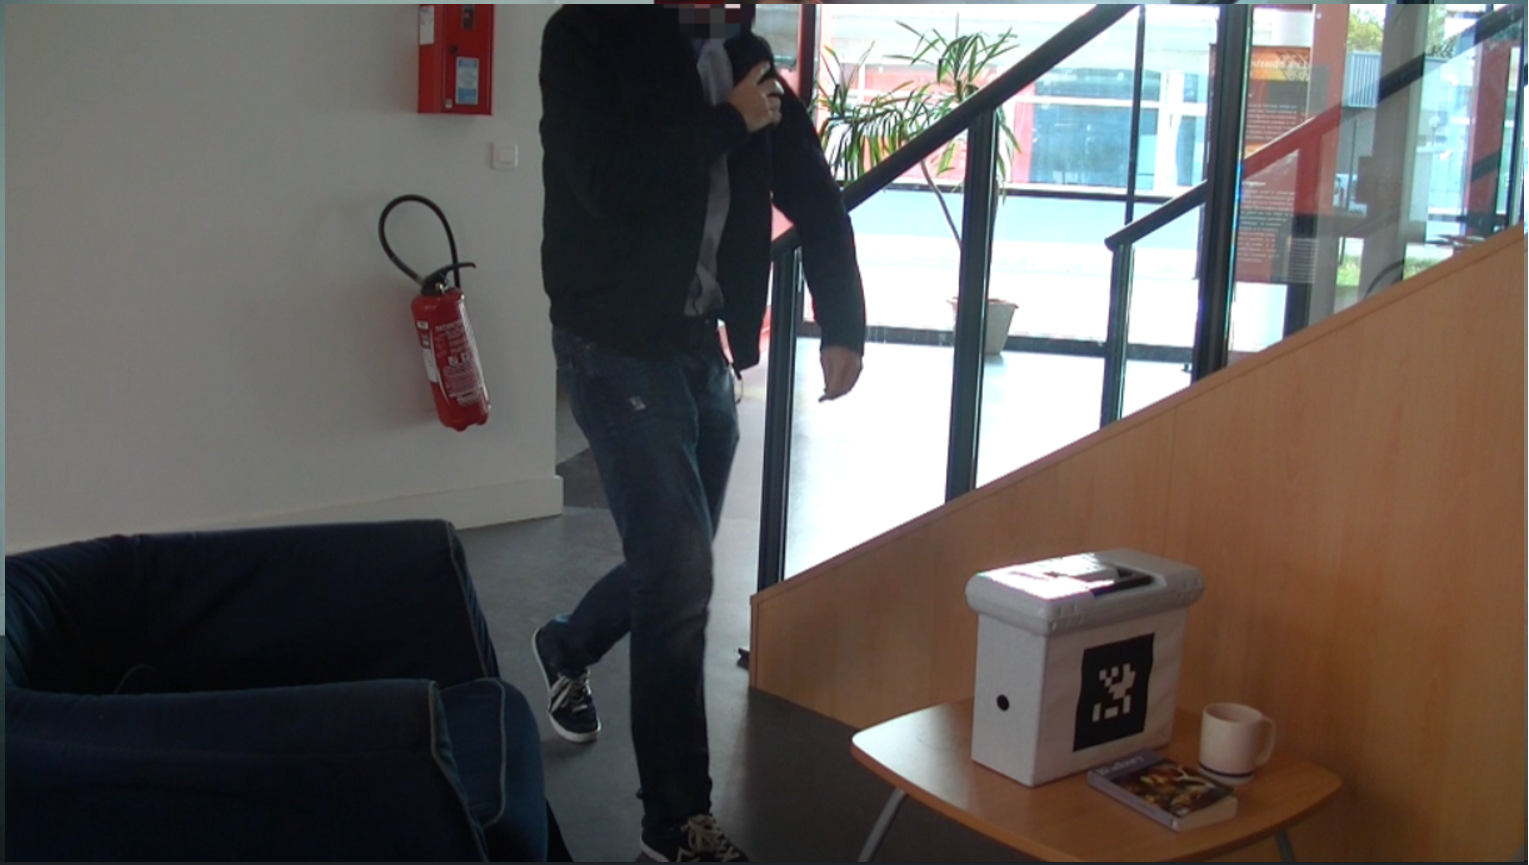
\includegraphics[scale=0.5]{img/situation_assessment/keys2-blur.pdf}
	\caption{The keys intention scenario}
	\label{fig:situation_assessment-keys}
\end{figure}

\subsection{User Study}
We built an online user study, where we presented videos related to the tests and events of the two scenarios to users, who had to evaluate the likelihood of each intentions of the scenario
on a five-level Likert scale. The user study was conducted in three languages, with users living in two different countries\footnote{A version of this user study was provided at http://goo.gl/forms/YiuFHnF63c}. We collected answers from 78 adults, performed an average, and converted them to percentile scores, in order to compare them with the robot's predictions.

Looking at users' answers (figure \ref{fig:situation_assessment-user_study_results}), we can see that, in the absence of clues, people rated similarly the two intentions related to visible objects. Contextual clues had the highest influence on users' ratings. This is particularly visible in the \textit{Contextual Clues} test of the \textit{Keys Scenario}, where users chose as the most likely intention \textit{Take Keys}, even if no keys were visible in the video. Divergent beliefs also influenced users decisions, but not as strongly as context. The strongest responses, over all, where given by the \textit{Divergent Belief Max} test on \textit{Keys Scenario}, which uses both divergent belief and contextual information.

\subsection{Robot implementation}
At the start of a scenario the robot scanned the environment, building a model of its world state. With our perception capacities, we can not detect if the cookie box is full or empty, and so we consider it as full at the start of a test, and update its value using the $postconditions$ of inferred human actions. We consider the box as empty when we infer that a human has taken a cookie from inside, and as full when we infer that a human has put a cookie in it.

We built different IGs for the scenarios. Each test had a different graph, related to its main agent. We considered three different Context Nodes for these IGs: $Hot Day$, true when the day is particularly warm; $Break Time$, true when the agents are taking a pause; $Time to Leave$, true when it's late in the day, and the humans usually leave work and return home.

As previously said, we chose to follow \cite{Liu2014} in order to learn the link between Contexts and Intentions. We created a second user study with 15 users, in which we presented a set of 5 scenarios, each one related to one of the intentions of our tests. For each scenario we asked the users to rate the perceived link, on a five-level Likert scale, between the intention and our three contexts. We averaged users' answers and calculated the conditional probabilities between context nodes and intention nodes from these averages.


In the \textit{Cookie Scenario} the graph for the tests is constructed from the following nodes:
\begin{itemize}
\item Context Nodes: \textit{Hot Day}, \textit{Break Time}, \textit{Time to Leave}
\item Intention Nodes: \textit{Fill Cookie Box}, \textit{Eat Cookie}, \textit{Drink Water}, \textit{Read Book}.
\item Action Nodes: \textit{Move to Table}, \textit{Move to Kitchen}.
\item Observation Nodes: distance of the agent body and hand to each action's associated \textit{target}.
\end{itemize}

We introduce the \textit{Fill Cookie Box} intention, not present in the human test, to allow the robot to detect when Bob fills the \textit{Cookie Box} during the \textit{Divergent Belief Event}.

Our robot doesn't have speech recognition capacities. We simulated this capacities, and set Context Nodes to plausible values, that could be extracted by watching the videos. For the \textit{Contextual Clues} test, we set the value of \textit{Hot Day} to true (since Max is commenting about the temperature), and \textit{Break Time}, and \textit{Time to Leave} to false (since no data in the video points to one of these contexts being true. Max and Bob seem to have taken a break from work before the other events are shown, in the Divergent Belief Event).
%Our robot doesn't have speech recognition capacities. and for \textit{Contextual Clues} test, set the value of \textit{Hot Day} to \textit{true}, and the value of \textit{Break Time} to \textit{false}, i.e. the robot knows that it is not the usual time for the agents to take a break.

\textit{Divergent Belief Event}, \textit{Divergent Belief Max}, and \textit{Divergent Belief Bob} were showed sequentially to the robot, which updated the agents' mental models and created new IGs accordingly. During the \textit{Divergent Belief Event} several IGs need to be created with different action and observation nodes, to follow the sequence of actions by the two agents. For example, when \textit{Max} leaves the room, \textit{Bob} has the possibility to execute the actions \textit{Take Mug}, \textit{Take Water Bottle}, \textit{Open Cookie Box}, \textit{Move to Kitchen Shelf} or \textit{Leave Room}. Intention and Context nodes remains the same in all the IGs of the scenario.


The \textit{Keys Scenario} has a similar IG, with the following differences.
\begin{itemize}
\item Context Nodes: \textit{Hot Day}, \textit{Break Time} and \textit{Time to Leave}.
\item Intention Nodes: \textit{Drink Water}, \textit{Take Keys}, \textit{Read Book}.
\end{itemize}

Action Nodes and Observation Nodes are the same as the previous scenario, and follow the same ideas during the \textit{Divergent Belief Event}. An example of IG used in the tests can be seen in figure \ref{fig:situation_assessment-intention_graph}. For the \textit{Contextual Clues} and \textit{Divergent Belief} test, we set the \textit{Time to Leave} context value to \textit{true} (since Max is putting a coat and seems in a hurry), and other context node values to \textit{false}. Using the component described in the previous sections, and these IGs the robot was able to obtain predictions from the user actions.

\subsection{Discussion}
\label{sec:discussion}
We performed TOST tests for each intention in the scenarios, comparing the humans' answers with the robot's, for a total of 21 tests. We calculated p-values and performed our tests using a significance value $\alpha=0.05$.

Analyzing the results of our equivalence tests, shown in figure \ref{fig:situation_assessment-user_study_results}, produces some interesting information.
\begin{itemize}
\item The behavior of our system is often close to human capacities. 19 tests out of 21 passed our requirements for significance level, often with very low p-value scores. 
\item Context and Divergent Belief are necessary. A system without these skills would only have been able to model properly the \textit{No Clues} cases. 
\item There are still some missing aspects in our system. We failed to reject the null hypothesis for two tests. In \textit{Divergent Belief Bob} users rated higher the \textit{Eat Cookie} intention than the \textit{Drink Water} intention, possibly because they thought that since \textit{Bob} filled the \textit{Cookie Box} he may want to eat a \textit{Cookie}. This makes us think that humans use deep temporal reasoning to evaluate intentions, considering the whole history of actions performed by agents.  
\end{itemize}
 \begin{figure}[ht!]
	\centering
	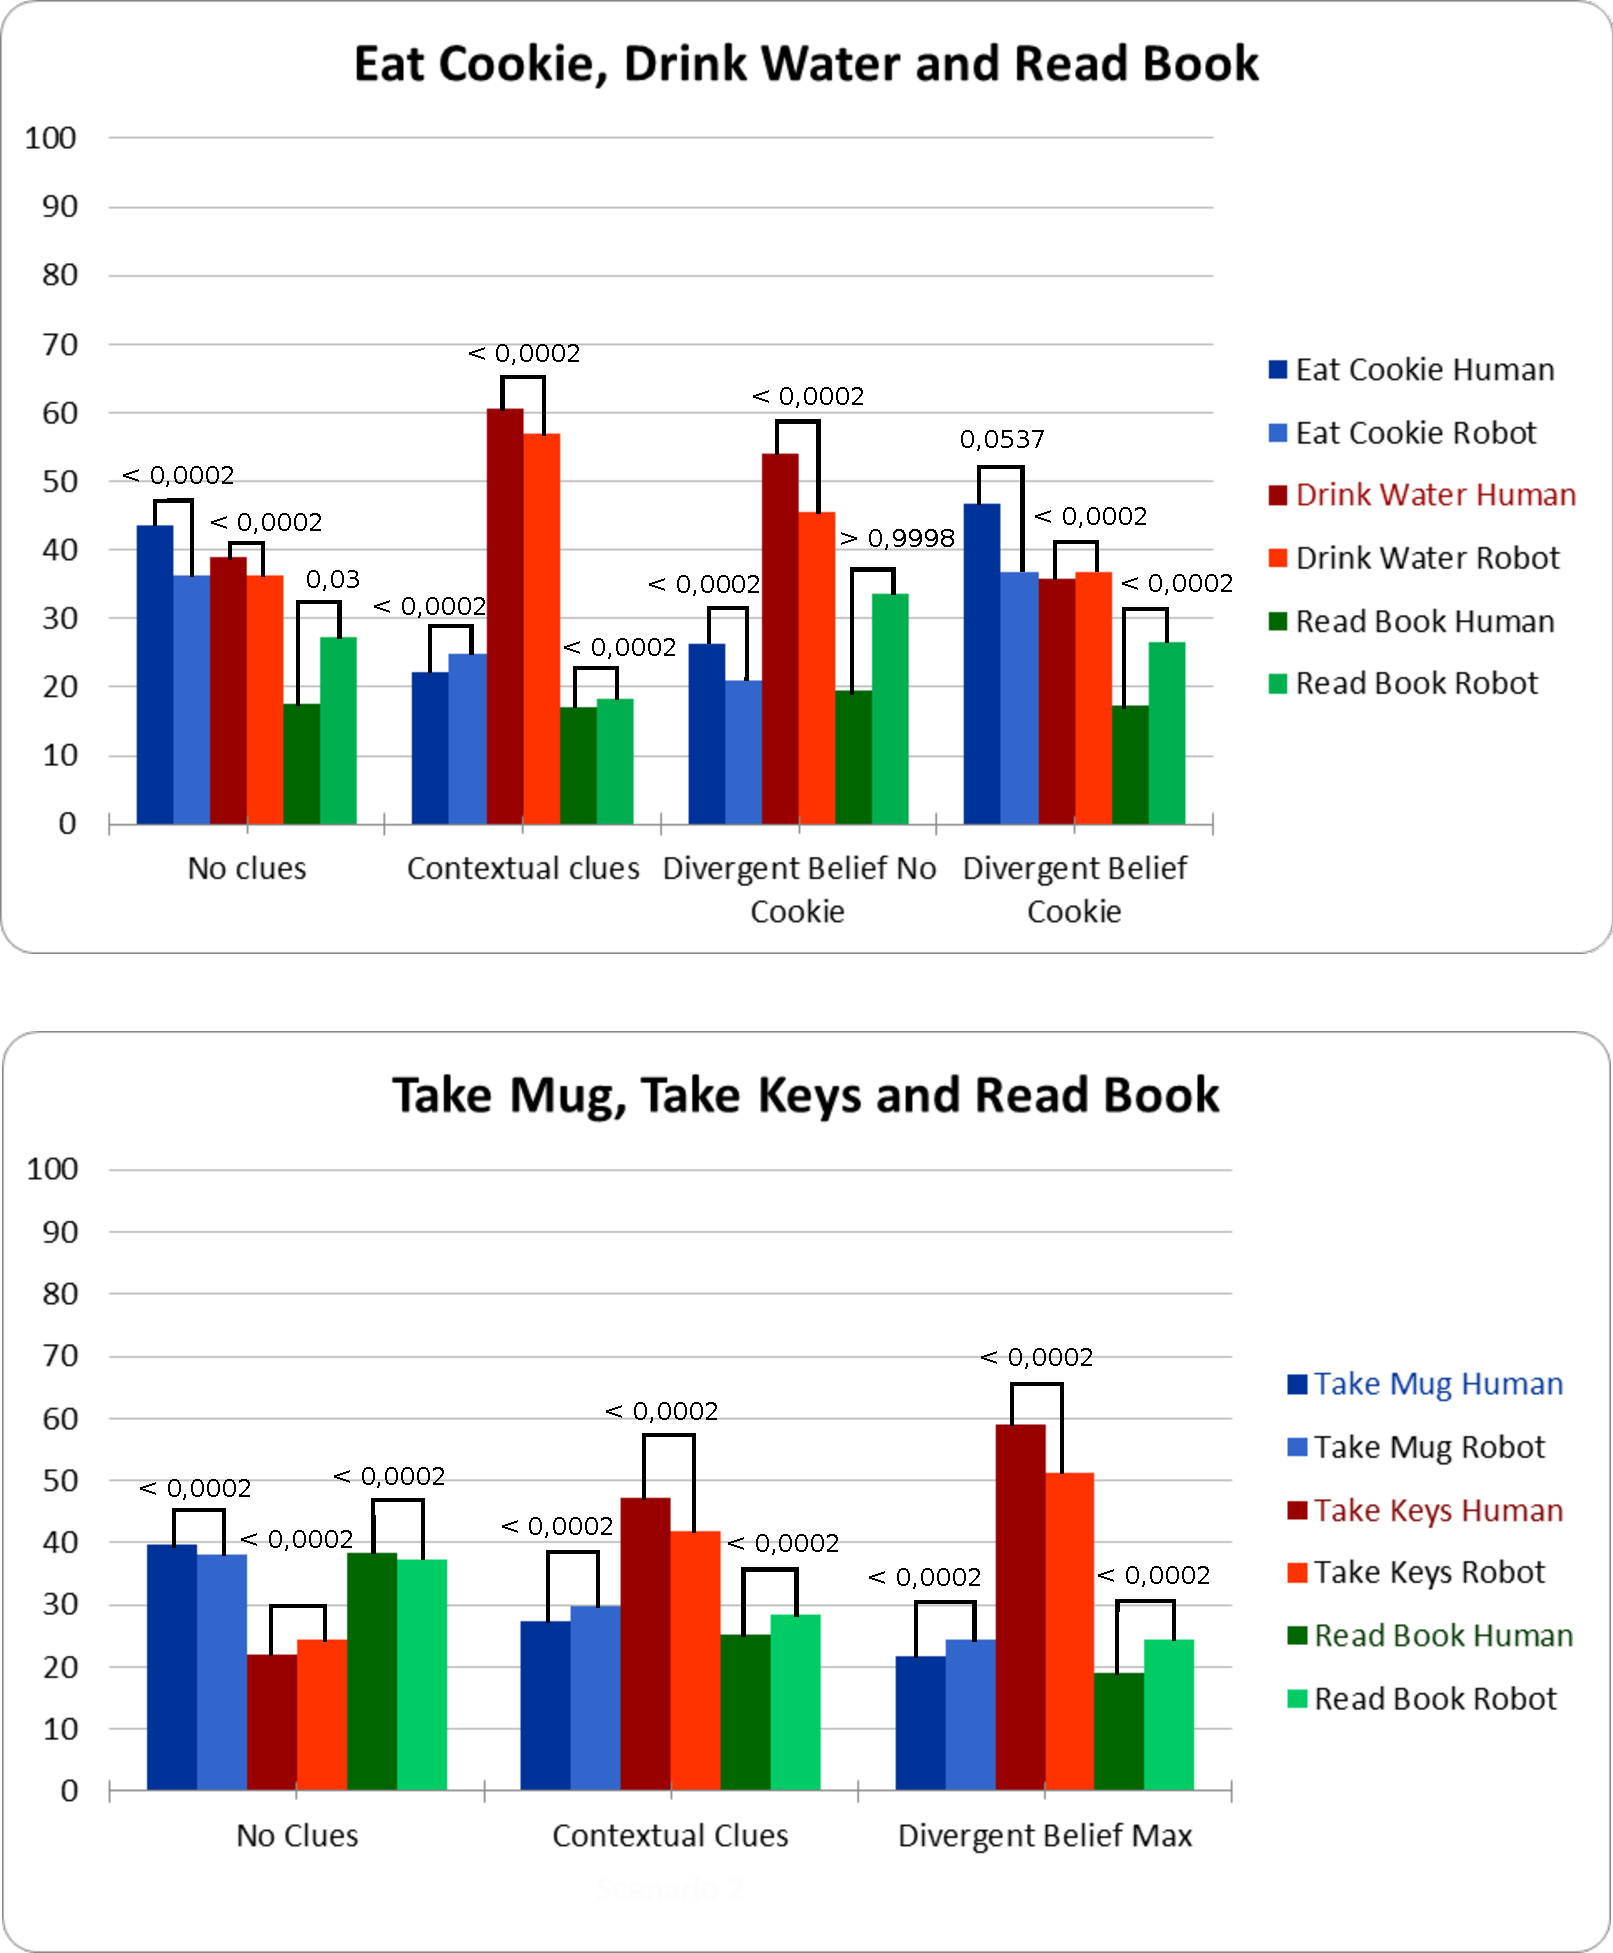
\includegraphics[clip,scale=0.5]{img/situation_assessment/pvalues1.pdf}
	\caption[Experiment results]{Experiment results. Results from the two scenarios are represented as graphs. Intentions, as estimated by the humans and the robot, are represented by different colors, as shown in the legend of the graphs, with estimations of the same intention by the robot or the human placed in adjacent position. Each column represents the likelihood of an intention, expressed as a percentile score. P-values from the equivalence tests are shown, linking the estimation of an intention by the humans and by the robot.}
	\label{fig:situation_assessment-user_study_results}
\end{figure}



